
\chapter{Literature Study}

  \section{Password habits among users}

    The term ``habit'' is often a bad thing when talking about security. A habit is often hard to change and are often a predictable pattern. Password reuse is one of the known password habits among users. It is a well known problem that users tends to have an increasingly number of account that requires the users to remember yet another number of password across multiple systems and devices. The problem is not just to remember all the password needed, but also remembering which passwords that belongs to which account or device. Because of the human capacity of remembering password are causing users to choose weak passwords, as well as reuse the passwords across multiple web pages. In order to understand the users passwords habits, this section will include relevant research on users passwords habits.

    \subsection{Password habits among web users}

      %Password reuse, frequency of webpage use (login habits), password strength, password policy

    One of the first large-scale studies on web password habits was conducted in 2007 by Microsoft research \cite{habits1}. They analyzed web password habits among 544960 web users over a period of 3 months. The data was collected from a Windows Live Toolbar and they observed activities like login frequency. They also collected information about the users age, the strength of the users passwords, as well as number of unique passwords and its use across different URLs. They observed that a normal user have an average of 7 distinct password and that an average of 5 of these password was re-used on different web pages. The estimate on average number of account pr user was estimated to be 25 account pr user, but this would probably be higher since it 7 years ago. 

    Password habits may be different across different subpopulation in cause of different background or culture. In 2012 Joseph Bonneau released a analysis of 70 million passwords from Yahoo! \cite{Bonneau2}. The data is analyzed in terms of guessing rate by using a dictionary attack. The collected data contained 328 subpopulations. The results showed that there was no ``good'' populations among the collected data, but there was a variation in the population. Demographically, the gender had a small effect in the guessing rate, but it showed that age tended to give effect where password strength increases across different age groups. The analysis also showed that language had a significantly effect on the password strength where Indonesian-speaking users were among the weakest subpopulations, and in contrast the German and Korean-speaking users provided relatively stronger passwords. 

    Passwords are not just used in our private life, but also a requirement in a critical concern from a business point of view where the use of authentication for corporate systems, mobile, and room codes plays a major role in normal day of work. In corporate systems users are often promt with the a notification forcing them to change the password in a specified time interval. The problem with this is that user already have problems remembering their passwords as is. A research group conducted a questionnaire survey in a large organization \cite{habits2}. The goal was to get a understanding of password habits in a business point of view. The results showed that the users were prompt with password change 7 times a year causing 68\% of the employees to re-use the same password with a minor change in order to still be able to remembering their passwords.

    \subsection{Security habits among smartphone users}

    %Intro
    Users are not only dependent on remembering passwords across multiple web pages and systems, but do also need to remember passwords for our small mobile devices. In todays society we're addicted to our mobile devices in our every day life. Mobile devices are not just a communication tool for calling and texting, but also an important tool for every day tasks like doing our work, reading mail, pay our bills and keeping up with our social life. This trend makes our mobile devices vulnerable in terms of security. To avoid unwanted access, smartphones offers different locking mechanisms. The history of locking mechanisms was often a solution solely to prevent accidental use, while current mobile phones require protection in order to secure the potentially vast amount of private data that we keep on our smartphones. Our mobile devices are in rapidly use, leading users to create and reuse shorter passwords and PINs, or no authentication at all. 

    % The time used on unlocking the phone
    In terms of security it is interesting to look at the use of mobile devices and look at the locking habits among users on mobile devices. It is known that services that are rapidly used have weaker password because of the overhead the user needs to spend on typeing their password. In 2014 a group of researchers published a field study of smartphone (un)locking behavior \cite{habits3}. Some of the problems with smartphone users tends to be their rapidly use of their phone. When the device are rabidly use, it results in a lot of time unlocking their phone between every use. In the study they found that there was a significant overhead in the time used of unlocking their phone, where the users participated in the field study used 2.9\% (9\% in the worst case) of their time unlocking their smartphone. 
    
    % The use of locking mechanisms
    Smartphones in use today do not require their users to have a locking mechanism on their smartphone. It is well known that users tends to choose to easiest way out and may result in the choice of not having any locking mechanism at all. Based on the result of the overhead in time used on unlocking their phone, a result may be to take the easiest way out by ignoring the vulnerability of not using a locking mechanism at all. It have been discovered that over 40\% of the users only used a basic ``slide-to-unlock'' mechanism on their smartphone, as well as over 16\% didn't use any locking mechanisms at all \cite{habits3}. This highlights a major bad habit among mobile users. What happens if your mobile is stolen? 

    % Risk vs securtiy
    It is important to understand why people use or not use locking mechanisms on their smartphone. Research have covered that the 46.8\% of the participants agreed or fully agreed that unlocking their phone can be annoying, but at the same time 95.5\% of the somewhat or fully agreed that they liked the idea that their phone was protected \cite{habits3}. This highlights that the users wants to be secure, but there might be a trade-off between the time used to unlock the smartphone vs the security risk.


    \subsection{Graphical password habits among users}

      %Quantifying the security of graphical passwords: the case of android unlock patterns
      %Patterns in the Wild: A Field Study of the Usability of Pattern and PIN-based Authentication on Mobile Devices
      %How many looses their phones?
      %How much do users use their phone (measured in hours)?


  \clearpage
  \section{Graphical passwords}

    %Oppsummere forskning på grafiske passord, dermed gå direkte inn på forskning på de forskjellige OS'ene. Må da beskrive sikkerhet på de forskjellige OS'ene i bakgrunnsteori. Passer best inn under bakgrunnsteori fordi det bare er oppramsing av fakta.

    %OBS! I denne seksjonen må det legges til flere kilder!

    Authentication with text-based passwords are a common approach, but it is well known that users often choose weaker passwords because of the limitations of recalling text-based passwords. Graphical passwords came as an alternative solution for overcoming the limitations of text-based passwords, and was inspired by researchers that showed that the graphical memory of humans is particularly well-suited to remember graphical information. 
    Like text-based passwords schemes, graphical password schemes are also a knowledge-based authentication scheme, e.g. ``something you know'' that are described in the background theory. Since it all started around 1999, there have been many suggestions for graphical password schemes. 

    \begin{wrapfigure}{l}{0.35\textwidth}
      \vspace{-20pt}
      \begin{center}
        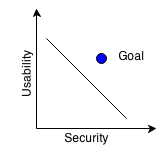
\includegraphics[scale=0.7]{pics/UsabilityVsSecurity.png}
      \end{center}
      \vspace{-20pt}
      \caption{Usability vs. Security}
      \vspace{-10pt}
    \end{wrapfigure}

    The problem with graphical password schemes is that they often promise improved password memorability and thus usability, while at the same time improving the security \cite{Biddle}.Since the first graphical password schemes was proposed, it is not widely in use. One of the problems with graphical approaches are that they require more overhead in the authentication phase. Like text-based passwords the users can simply type their passwords, while many of the graphical passwords require to go through many steps, requiring the user to spend more time in the authentication phase. The graphical password schemes like Passface and grIDsure are some of the graphical password schemes with commercial interest, while on mobile devices graphical passwords are not widely adopted. There is a known problem with authentication on mobile devices because of the difficulty of typing on mobile keyboards, making authentication schemes using alternatives getting increased attention. Because of the difficulty of writing on mobile keyboards it highlights the importance of understanding the usability and security implications.

    In many years, the field of psychology been a important in order to understand how humans interpret and remember different information. Psychology studies have recognized that the human brain have a superior memory for recognizing and recalling visual information rather recognizing and recalling verbal or textual information. One known theory is the ``dual-coding theory'', suggesting that verbal and non-verbal memory are processed and represented differently in humans mind. Text are verbal information that is represented symbolically, in contrast to non-verbal information like images that are mentally represented in a way that perceived concepts are assigned to a perceived meaning of what is directly observed. Both verbal and non-verbal information can be used when recalling information. For example, say a person have received stimulus of the concept ``cat'', both the image of a cat as well as the word ``cat''. When the person is asked to recall the concept ``cat'', the person can retrieve the image or the word individually, or both simultaneously. 
    If the word ``cat'' is recalled, the image of the cat is not lost and can still be retrieved at a later point in time. The ability to code a stimulus in two different ways can increase humans ability to remember, in contrast to only code the stimulus in one way.
    In the background theory there are described three different categories of graphical passwords according to the memory task involved in remembering and entering the password, e.g. recall, recognition and cued-recall. 

    %SETT INN ILLUSTRASJON AV KATT

     %Photos are mentally represented in that perceived traits that are observed and assigned to a perceived importance based on what is directly observed.
    %Bilder er mentalt representert på den måten at oppfattede trekk som blir observert og er tilårdnet en oppfattet betydning basert på hva som blir direkte observert.

    In terms of authentication, its primary goal is to provide security for its intended environment in order to avoid security attacks. In knowledge-based authentication, e.g. ``something you know'', we classify attacks into two general categories: guessing and capturing attacks. In a guessing attack the attackers are able to search through the entire password space, or either predict the users passwords patterns in order to avoid searching through the whole passwords space (often referred to as a dictionary attack). When talking about capturing attacks, the attackers are directly obtain the passwords by observing the authentication process. One of the known capturing attacks on graphical passwords are shoulder surfing because of its graphical visualization. 

    %One Graphical Password scheme that are widley adopted on mobile devices are the Android Unlock Pattern that are a variation of the graphical password scheme PassPoint. 

    %Mobile dec





 
    